\documentclass[a4paper, 12pt]{article}  %set doc type and font size
\usepackage{fontspec}

% math tools
\usepackage{amsmath}
\usepackage{amssymb}
\usepackage{amsfonts}

% 序列標號
\usepackage{enumerate}

% 導入圖形與表格的封包
\usepackage{graphicx}
\usepackage{booktabs}
\usepackage{tikz}
\usetikzlibrary{arrows.meta, positioning, shapes.geometric}

% set chinese
\usepackage{xeCJK}
\xeCJKsetup{AutoFakeBold=true, AutoFakeSlant=true}
\setmainfont{Times New Roman}
\setCJKmainfont{標楷體}
\XeTeXlinebreaklocale "zh"
\XeTeXlinebreakskip = 0pt plus 1pt

\title{Chapter 2　Assignment \small{Due date: March 30, 2026 (Mon)}}
\author{黃丞暘　611211106}
\date{}

\begin{document}
\maketitle % 顯示標題區塊

\section*{2.1}
\textbf{Sol.}
    \begin{enumerate}[i.]
        \item 
        $$
        f(x)=F'(x)=\begin{cases}
            \dfrac{1}{b-a}, 
            & a\le x\le b\\
            1, & \text{o.w.}
        \end{cases}
        $$
        \item 
        \begin{align*}
            E(X) &= \int_{-\infty}^{\infty} x f(x)\,dx
            = \int_a^b x \cdot \frac{1}{b-a}dx
            = \frac{1}{b-a}\int_a^b xdx \\[6pt]
            &= \frac{1}{b-a}\left[\frac{x^2}{2}\right]_a^b
            = \frac{1}{b-a}\cdot \frac{b^2-a^2}{2}
            = \frac{a+b}{2}
        \end{align*}
        \begin{align*}
            E(X^2) &= \int_{-\infty}^{\infty} x^2 f(x)\,dx
            = \int_a^b x^2 \cdot \frac{1}{b-a}dx
            = \frac{1}{b-a}\int_a^b x^2dx \\[6pt]
            &= \frac{1}{b-a}\left[\frac{x^3}{3}\right]_a^b
            = \frac{1}{b-a}\cdot \frac{b^3-a^3}{2}
            = \frac{a^2+ab+b^2}{3}
        \end{align*}
        \begin{align*}
            Var(X) &= E(X^2)-[E(X)]^2
            = \frac{a^2+ab+b^2}{3}-\left(\frac{a+b}{2}\right)^2
            = \frac{(b-a)^2}{12}
        \end{align*}
        \item 
        \begin{itemize}
            \item The pdf is constant on $[a, b]$, so all values in the interval are equally likely.
            \item The grave of pdf is a rectangle over the interval $[a, b]$.
        \end{itemize}
        \item $$P(7\le X\le 9)=\frac{9-7}{10-5}=\frac{2}{5}=0.4$$
    \end{enumerate}

\section*{2.6}
\textbf{Sol.}
    $$X\sim Bin(n=10, p=0.2)$$
    $$f_X(x)=\begin{pmatrix}
        n \\
        x 
    \end{pmatrix}p^x(1-p)^{n-x}$$
    \begin{enumerate}[i.]
        \item $$E(X)=np=10\cdot 0.2=2$$ $$Var(X)=np(1-p)=2\cdot (1-0.2)=1.6$$
        \item 
        \begin{align*}
           P(3\le X \le 5) &= P(X=3)+P(X=4)+P(X=5) \\
            &= {\begin{pmatrix} 10 \\ 3 \end{pmatrix}}(0.2)^3(0.8)^7
            +{\begin{pmatrix} 10 \\ 4 \end{pmatrix}}(0.2)^4(0.8)^6
            +{\begin{pmatrix} 10 \\ 5 \end{pmatrix}}(0.2)^5(0.8)^5 \\
            &\approx 0.3158
        \end{align*}
    \end{enumerate}

\section*{2.8}
\textbf{Sol.}

10, 12, 15, 17, 20, 20, 23, 25, 28, 30,
40, 43, 45, 48, 50, 50, 59, 61, 64, 70.
    \begin{enumerate}[i.]
        \item 
        $20\cdot \dfrac{1}{4}=5\Rightarrow Q_1=\dfrac{a_5+a_6}{2}=\dfrac{20+20}{2}=20$
        
        $20\cdot \dfrac{1}{2}=10\Rightarrow Me=\dfrac{a_10+a_11}{2}=\dfrac{30+40}{2}=35$

         $20\cdot \dfrac{3}{4}=15\Rightarrow Q_3=\dfrac{a_15+a_16}{2}=\dfrac{50+50}{2}=50$
        \item $IQR=Q_3-Q_1=50-20=30$
        \item
        $\text{Lower bound} = Q_1-1.5IQR=20-45=-25$
        
        $\text{Upper bound} = Q_3+1.5IQR=50+45=95$

        \begin{figure}[htbp]
        \centering
        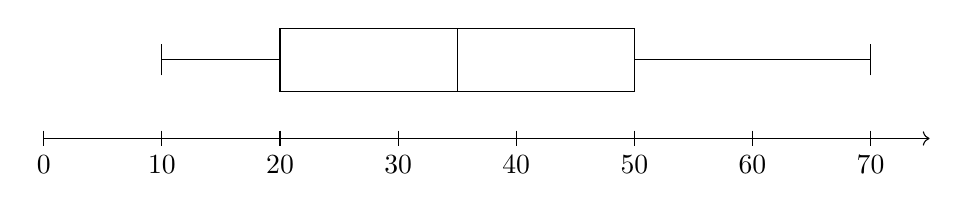
\begin{tikzpicture}[x=0.15cm,y=1cm]
            % number line
            \draw[->] (0,0) -- (75,0);
            \foreach \x in {0,10,20,30,40,50,60,70}
                \draw (\x,0.1) -- (\x,-0.1) node[below] {\x};

            % whiskers
            \draw (10,1) -- (20,1);
            \draw (50,1) -- (70,1);

            % box
            \draw (20,0.6) rectangle (50,1.4);

            % median
            \draw (35,0.6) -- (35,1.4);

            % whisker ends
            \draw (10,0.8) -- (10,1.2);
            \draw (70,0.8) -- (70,1.2);
        \end{tikzpicture}
        \end{figure}
    \end{enumerate}

\section*{2.9}
\textbf{Sol.}

D, D, R, O, R, R, R, D, R, D, D, R, D, D, R, R, R, O, D, D
\begin{enumerate}[i.]
    \item \mbox{}\\
    \begin{tabular}{c|c|c}
        \hline
        Political Status & Frequency & Relative Frequency \\
        \hline
    $D\ (\text{Democrats}) $ & 9 & 0.45 \\
    $R\ (\text{Republicans})$ & 9 & 0.45 \\
    $O\ (\text{Others})$ & 2 & 0.10 \\
        \hline
    \end{tabular}
    \item \mbox{}\\
    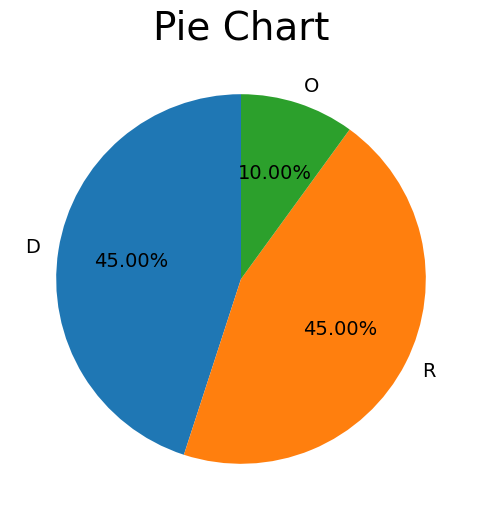
\includegraphics[width=0.8\linewidth]{2.9pie.png}
    \item \mbox{}\\
    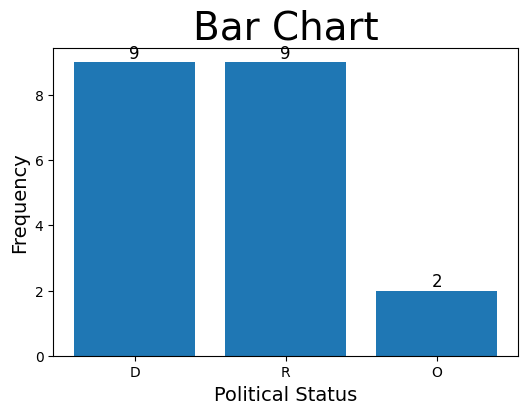
\includegraphics[width=0.8\linewidth]{2.9bar.png}
\end{enumerate}



\section*{2.11}
\textbf{Sol.}
\begin{enumerate}[i.]
    \item \mbox{}\\
    \begin{tabular}{c|c|c|c}
        \hline
        Class Interval & Frequency & Relative Frequency & Density\\
        \hline
    $[5,10)$  & 20 & 0.0615 & 0.0123\\
    $[10,15)$ & 45 & 0.1385 & 0.0277\\
    $[15,20)$ & 75 & 0.2308 & 0.0462\\
    $[20,25)$ & 90 & 0.2769 & 0.0554\\
    $[25,30)$ & 60 & 0.1846 & 0.0369\\ 
    $[30,35)$ & 35 & 0.1077 & 0.0215\\
        \hline
    \end{tabular}
    \item \mbox{}\\
    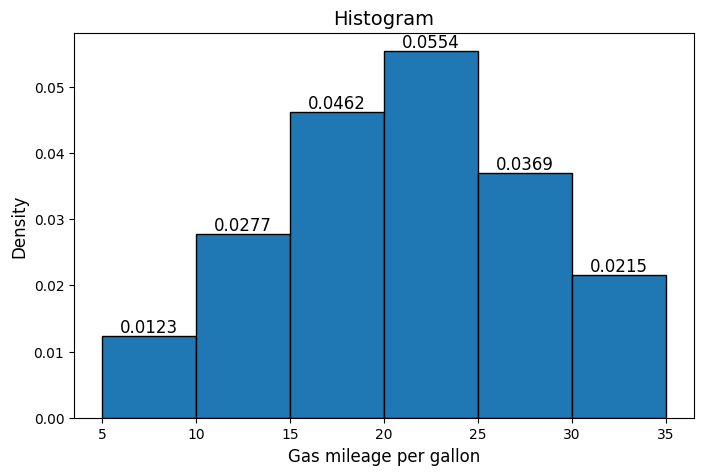
\includegraphics[width=1\linewidth]{2.11Hist.png}
    \item $$P(5\le X<20)=\frac{20+45+75}{325}\approx 0.4308$$
    

\end{enumerate}


\section*{2.14}
\textbf{Sol.}

\section*{2.19}
\textbf{Sol.}

\section*{2.21}
\textbf{Sol.}

\section*{2.25}
\textbf{Sol.}

\section*{2.26}
\textbf{Sol.}

\end{document}